\documentclass{beamer}

\usetheme{Madrid}
\usecolortheme{seahorse}
\usepackage{multirow}
\usepackage{caption}
\setbeamertemplate{navigation symbols}{}
\useinnertheme{rectangles}
\usepackage{varwidth}

\usepackage{appendixnumberbeamer}
\usepackage[ruled, vlined, longend]{algorithm2e}
\beamertemplatenavigationsymbolsempty
\usepackage[many]{tcolorbox}
\usetikzlibrary{decorations.pathmorphing}
\usetikzlibrary{shadows}
\usepackage[absolute,overlay]{textpos}
\usepackage{listings}
\lstset {
  backgroundcolor=\color{white},
  basicstyle=\ttfamily\footnotesize,
  numbers=left,numberstyle=\tiny,numbersep=5pt,
  emph={proc, fun, let, send, consume, global, type, record, if, else,
    in, not, foldt, return, on, ordering, by, as, or },
  emphstyle={\bfseries},
  literate = {=>}{{\bf=>}}2
}
\usepackage{graphicx,accents,pinlabel}

\definecolor{paper}{RGB}{239,227,157}
\newtcolorbox{tornpage}{%
    enhanced jigsaw, breakable, % allow page breaks
    frame hidden, % hide the default frame
    overlay={%
        \draw [
            fill=paper, % fill paper
            draw=paper!50!black, % boundary colour
            decorate, % decoration
            decoration={random steps,segment length=2pt,amplitude=1pt},
            drop shadow, % shadow
        ]
        % top line
        (frame.north west)--(frame.north east)--
        % right line
        (frame.north east)--(frame.south east)--
        % bottom line
        (frame.south east)--(frame.south west)--
        % left line
        (frame.south west)--(frame.north west);
    },
    % paragraph skips obeyed within tcolorbox
    parbox=false,
}
%\useoutertheme{default}
%\useinnertheme{rounded}

\titlegraphic{
\begin{center}
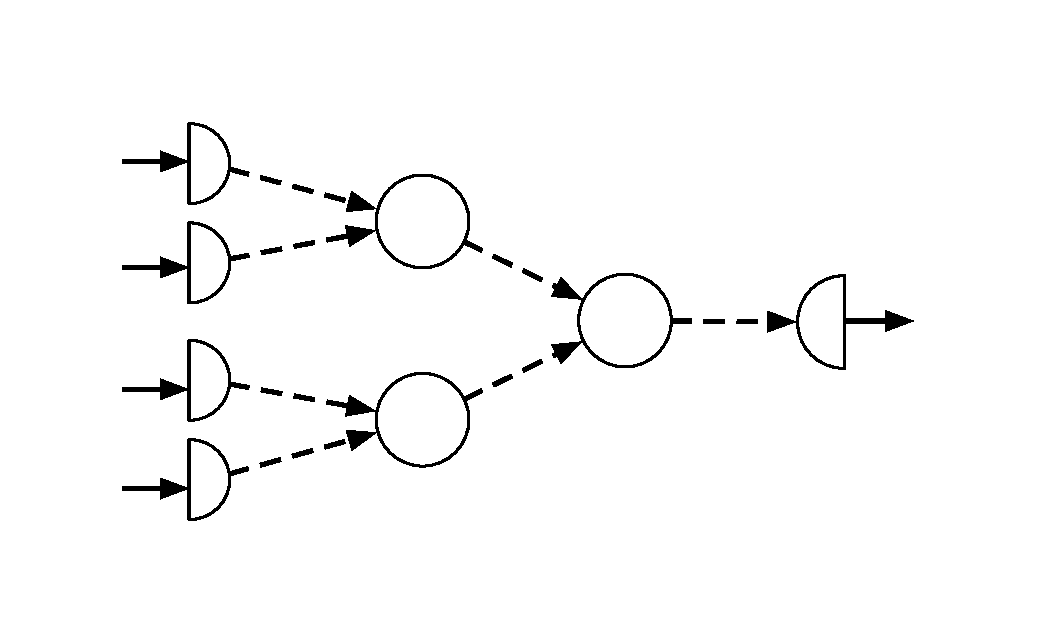
\includegraphics[width=3cm]{hadoop2}%
\end{center}
}

\usepackage{tikz}
\usetikzlibrary{shadows.blur}
\usetikzlibrary{shapes.symbols}
\usetikzlibrary{backgrounds}
\usetikzlibrary{arrows.meta}
\usetikzlibrary{shapes,snakes}
\usetikzlibrary{fit,calc,shadows}
\setbeamercolor{section in head/foot}{bg=white, fg=black}
%\beamertemplateshadingbackground{black!10}{blue!15}
\makeatletter
\setbeamertemplate{footline}
{
  \leavevmode%
  \hbox{%
  \begin{beamercolorbox}[wd=.333333\paperwidth,ht=2.25ex,dp=1ex,center]{section in head/foot}%
    \usebeamerfont{author in head/foot}\insertshortauthor~~\beamer@ifempty{\insertshortinstitute}{}{Richard G. Clegg}
  \end{beamercolorbox}%
  \begin{beamercolorbox}[wd=.333333\paperwidth,ht=2.25ex,dp=1ex,center]{section in head/foot}%
    \usebeamerfont{title in head/foot}{Studying Gab with Raphtory}
  \end{beamercolorbox}%
  \begin{beamercolorbox}[wd=.333333\paperwidth,ht=2.25ex,dp=1ex,right]{section in head/foot}%
    \usebeamerfont{date in head/foot}\insertshortdate{}\hspace*{2em}
    \insertframenumber{} / \inserttotalframenumber\hspace*{2ex} 
  \end{beamercolorbox}}%
  \vskip0pt%
}
\makeatother

\date[QMUL IADS]{Presentation to QMUL IADS}

\begin{document}


\frame{

\title[Raphtory]{A new tool for large temporal networks applied to the far right social network Gab}

\setcounter{framenumber}{0}

\begin{center}
\Huge{Raphtory: A new tool for large temporal networks applied to the far right social network Gab}


\vspace{0.2cm}

\inserttitlegraphic

\vspace{0.2cm}

\scriptsize{\raggedright
{\color{blue} Presenter: }Richard G. Clegg,  \\}
\scriptsize{\raggedright
%Work joint with the {\color{blue} Network-as-a-Service project}.  \\
{
    {\color{blue} Project team (alphabetical order): \\ }
Naomi Arnold, F\'{e}lix Cuadrado, Imane Hafnaoui, Raul Mondragon, Hugo Parada, Ben Steer }
}

%\tiny{(Prepared using \LaTeX \;and beamer.)}
\end{center}
}

\tikzset{onslide/.code args={<#1>#2}{%
  \only<#1>{\pgfkeysalso{#2}} % \pgfkeysalso doesn't change the path
}}
\tikzset{temporal/.code args={<#1>#2#3#4}{%
  \temporal<#1>{\pgfkeysalso{#2}}{\pgfkeysalso{#3}}{\pgfkeysalso{#4}} % \pgfkeysalso doesn't change the path
}}


\section{Introduction}


\tikzstyle{box} = [draw=black,shade, 
      font = \footnotesize,
      align= center,
      top color=blue!40,
      bottom color=blue!5,
      rounded corners=3pt,
      blur shadow={shadow blur steps=5}]

\tikzstyle{box2} = [draw=black,shade, 
      font = \footnotesize,
      align= center,
      top color=red!40,
      bottom color=red!5,
      rounded corners=3pt,
      blur shadow={shadow blur steps=5}]

\tikzstyle{net con} = [draw=black,ultra thick]

\frame{
    
    \frametitle{Aims of this talk (unordered list)}

\begin{block}{Aim A: Give insight into data}
What drives the evolution of the alt-right social network gab?
\end{block}
\pause
\begin{block}{Aim 1: Show a technique}
Temporal analysis and in particular ``windowing" is an invaluable tool for social network analysis. 
\end{block}
\pause
\begin{block}{Aim $\alpha$: Sell you a tool}
Raphtory is an open-source big-data platform developed at QMUL. It is unique in its ability to perform flexible temporal analysis on batch or streamed graph data
\end{block}
    
}

\frame{
    \frametitle{The gab platform (and why we care)}
\centering{
\begin{tikzpicture}%[show background grid]
\draw[white] (-5.5,-3.5) rectangle (5.5,3.5);
\node <1-> at (0,0) {
    {\begin{varwidth}{\linewidth}
\begin{itemize}
\item 95GB of raw data from the gab platform
\begin{itemize}
\item Data is user, posts (threaded), timestamps and other metadata.
\item NB our research on \alert{structure} not \alert{content}.
\end{itemize} 
\item First eighteen months of data available. 
\begin{itemize}
\item September 2016 -- May 2018.
\end{itemize}
\item Largely complete data from this period.
\begin{itemize} 
\item``free speech" focus means ``everything" is public.
\end{itemize}
\item Alt-right focus: 
\begin{itemize}
\item Racism, fake news, hate speech, radicalisation.
\end{itemize}
\end{itemize}
\end{varwidth}}
};
\node <2-> at (-2,0) {
\includegraphics[width=7cm,angle=20]{gab1}};
\node <3-> at (2,2) {
\includegraphics[width=8cm,angle=-10]{gab2}};
\node <4-> at (-2,1) {
\includegraphics[width=9cm,angle=-30]{gab4}};
\node <5-> at (-0,0) {
\includegraphics[width=7cm,angle=40]{gab3}};
\end{tikzpicture}
}


}



\frame{
    \frametitle{The Raphtory tool}
    
}

\frame{
    \frametitle{Social network analysis}
\begin{block}{Social network $\rightarrow$ graph $G$ }
We can form a graph from a social network by creating an edge between two users if they are friends or if they ``mention" each other.  
\end{block}
\pause
\begin{block}{Social network $\rightarrow$ many graphs $G(t,\tau)$}
There is no such thing as \alert{``the twitter graph"}. The graph varies hugely depending on the \alert{time} and \alert{timescale}.
\end{block}
}

\frame{
    \frametitle{Temporal graphs}
}

\section{Analysis}

\frame{
\frametitle{What drives growth on gab?}
\centering{
\begin{tikzpicture}%[show background grid]
\node<1> at (0,0){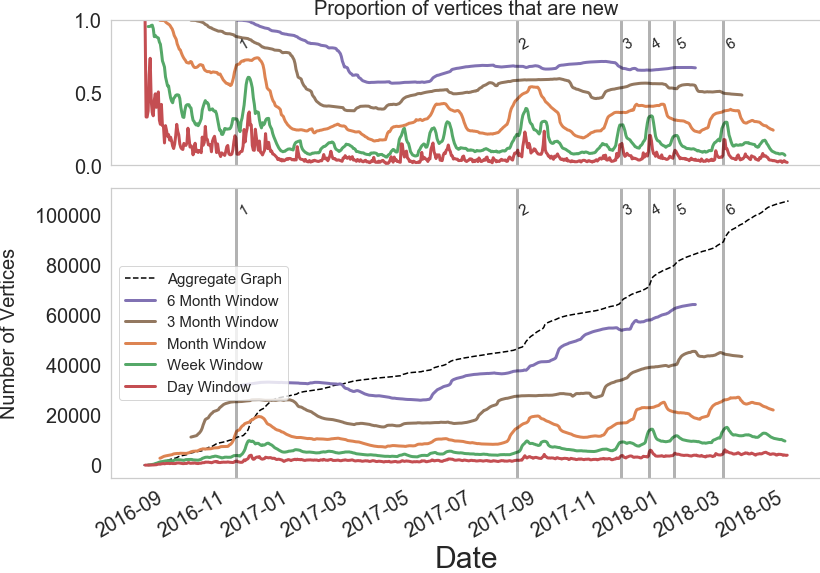
\includegraphics[width=\textwidth]{vertices}};
\end{tikzpicture}
}
}



\frame{
\frametitle{Is gab a ``social" network?}
\centering{
\begin{tikzpicture}%[show background grid]
\node<1> at (0,0){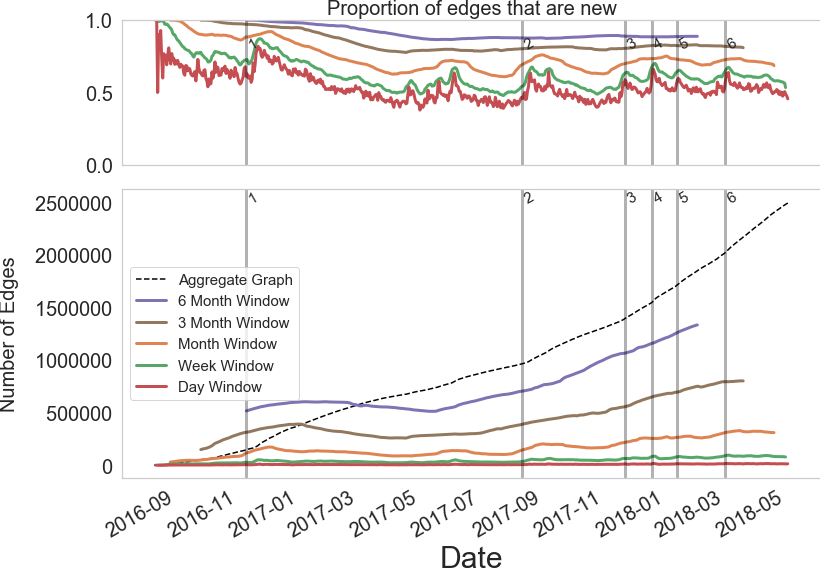
\includegraphics[width=\textwidth]{edges}};
\end{tikzpicture}
}
}

\frame{
\frametitle{Is gab a community?  Largest Connected Component}
\centering{
\begin{tikzpicture}%[show background grid]
\node<1> at (0,0){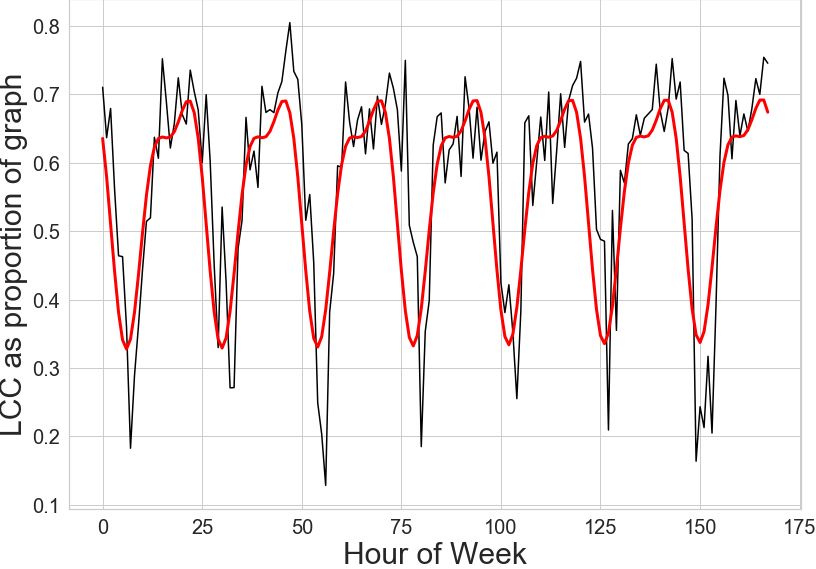
\includegraphics[width=0.8\textwidth]{lcc}};
\end{tikzpicture}
}
}

\frame{
\frametitle{Is gab a community?  Largest Connected Component}
\centering{
\begin{tikzpicture}%[show background grid]
\node<1> at (0,0){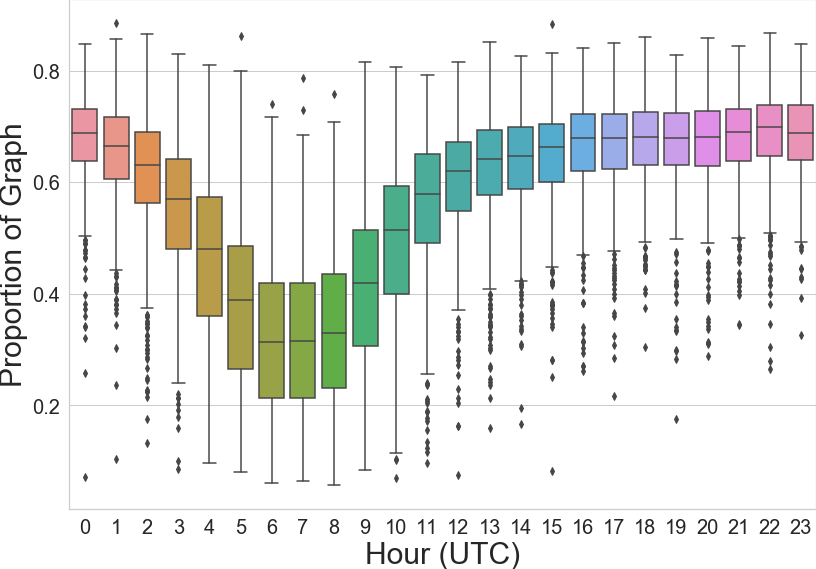
\includegraphics[width=0.8\textwidth]{prop_diurnal}};
\end{tikzpicture}
}
}


\frame{
    \frametitle{Is gab controlled by an ``elite"?}
\begin{itemize}
\item 
\end{itemize}
}

\frame{
    \frametitle{Is gab controlled by an ``elite"?}
\centering{
\begin{tikzpicture}%[show background grid]
\node<1> at (0,0){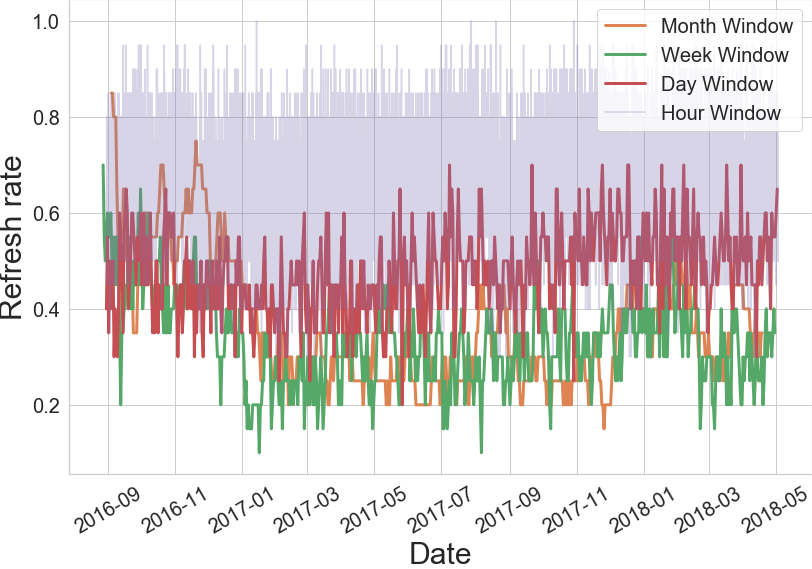
\includegraphics[width=0.8\textwidth]{jaccard}};
\end{tikzpicture}
}
}

\section{Conclusions}
\frame{
\frametitle{Conclusions (about gab)}    
\begin{itemize}
\item Long duration (months to years) gab is growing relatively slowly.
\begin{itemize}
\item Short duration (hours to days) we can witness rapid growth.
\item Growth driven by community specific events.
\end{itemize}
\item Gab is not a ``social" network -- interactions between ``strangers" not friends.
\item Analysed at the hourly level not always a ``connected" community
\begin{itemize}
\item Graph LCC shatters into disconnected pieces at off-peak hours.
\item This diurnal change of regime never observed before.
\end{itemize}
\item Are a cadre of elite users controlling users' attention? It depends on timescale.
\end{itemize}
}
\frame{
\frametitle{Conclusions (about Raphtory and temporal networks)}    
\begin{itemize}
\item Temporal networks provide a rich array of techniques that can get more out of your network data.
\begin{itemize}
\item Window based analysis provides many levels of insight. 
\item Akin to looking at frequency as well as time.
\pause
\end{itemize}
\item The Raphtory tool is a great way to look at temporal graph data.
\begin{itemize}
\item Funding from the Alan Turing Institute to develop it and analyse data.
\item Can help you use it on your data sets.
\item Bitcoin data, urban analytics, word semantics, other social networks.
\item Spin off company Chorograph developing it further.
\end{itemize}
\end{itemize}
}

\tikzstyle{cloudconn} = [draw=black, inner sep=0pt,
       line width=0.25mm,{Latex[length=2.5mm, width=1.5mm]}-{Latex[length=2.5mm, width=1.5mm]}]


\tikzstyle{platform} = [draw=black,shade, 
      anchor=south west,
      align= center,
      top color=blue!40,
      bottom color=blue!5,
      rounded corners=6pt,
      blur shadow={shadow blur steps=5},
      font = \footnotesize]
      

\frame{
\frametitle{Our Raphtory social network (a small subgraph)}
\centering{
\begin{tikzpicture}%[show background grid]
\draw[white] (-5,-3) rectangle (5,3);
\node <1-> [inner sep=0pt] at (-4.5,0.0) (fc) {
\includegraphics[width=1.5cm]{felix}};
\node <1-> [inner sep=0pt] at (4.5,0.0) (ih) {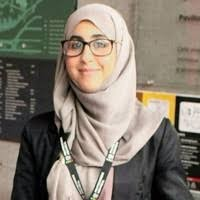
\includegraphics[width=1.5cm]{imane}};
\node <1-> [inner sep=0pt] at (-3,2.5) (bs) {
\includegraphics[width=1.5cm]{ben}};
\node <1-> [inner sep=0pt] at (3,2.5) (rc) {
\includegraphics[width=1.5cm]{rich}};
\node <1-> [inner sep=0pt] at (-3,-2.5) (rm) {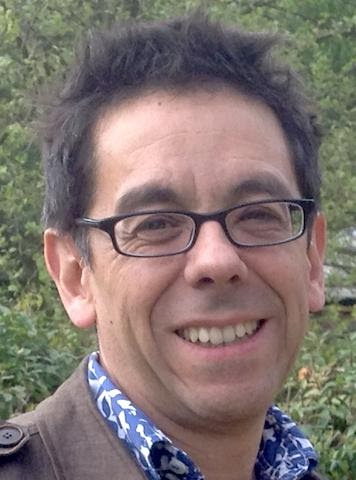
\includegraphics[width=1.5cm]{raul}};
\node <1-> [inner sep=0pt] at (3,-2.5) (na) {
\includegraphics[width=1.5cm]{naomi}};


\path[draw] <3-> (ih) edge[cloudconn] (fc);
\path[draw] <3-> (ih) edge[cloudconn] (bs);
\path[draw] <3-> (ih) edge[cloudconn] (rc);
\path[draw] <3-> (ih) edge[cloudconn] (na);
\path[draw] <3-> (ih) edge[cloudconn] (rm);
\path[draw] <2-> (fc) edge[cloudconn] (bs);
\path[draw] <2-> (fc) edge[cloudconn] (rc);
\path[draw] <2-> (fc) edge[cloudconn] (rm);
\path[draw] <2-> (fc) edge[cloudconn] (na);
\path[draw] <2-> (bs) edge[cloudconn] (rc);
\path[draw] <2-> (bs) edge[cloudconn] (na);
\path[draw] <2-> (bs) edge[cloudconn] (rm);
\path[draw] <2-> (na) edge[cloudconn] (rc);
\path[draw] <2-> (na) edge[cloudconn] (rm);
\path[draw] <2-> (rc) edge[cloudconn] (rm);
\node<4>[platform,anchor= south] at (0,0.1) {Paper on gab and temporal graphs \\
submitted to ICWSM 2020 (under review)
};
\node<4>[platform,anchor= north] at (0,-0.1) {Raphtory is on github \\https://github.com/miratepuffin/raphtory
};
\end{tikzpicture}
}
}
\end{document}
